\section{唯一性}
\label{sec:odeex-uniqueness}

漏斗状的多解出现在$\dot x=2\sqrt{\lvert x\rvert}$的零线上，那里右端随状态变化得太快。反过来想，什么样的右端能阻止两条解分开？设$\bm{u},\bm{v}$是同一初值的两条解，它们的差的变化率是$\bm{f}(t,\bm{u})-\bm{f}(t,\bm{v})$。若这个量能用差本身来控制，两条解一开始重合，就没有东西推动它们分开。

\paragraph{状态方向的Lipschitz条件}
把“右端的变化能用状态差控制”写成条件。下面只比较同一时刻的两个状态，时间方向没有光滑性要求。

\begin{definition}[状态方向的局部Lipschitz条件]
\label{def:odeex-local-lipschitz}
设$\bm{D}\subseteq\mathbb{R}\times\mathbb{R}^{n}$开，$\bm{f}:\bm{D}\to\mathbb{R}^{n}$。若对每点$(t_\ast,\bm{x}_\ast)\in\bm{D}$，存在它的邻域$\bm{U}\subseteq\bm{D}$和常数$L\geq0$，使对$\bm{U}$中所有同一时刻的两点$(t,\bm{x}),(t,\bm{y})$都有
\begin{equation}
 \lVert\bm{f}(t,\bm{x})-\bm{f}(t,\bm{y})\rVert_2\leq L\lVert\bm{x}-\bm{y}\rVert_2,
 \label{eq:odeex-lipschitz}
\end{equation}
就称$\bm{f}$在状态方向\term{局部Lipschitz连续}（locally Lipschitz continuous），且该性质对时间局部一致。
\end{definition}

定义里的“局部一致”指同一个$L$对邻域内所有时刻都有效。几何上，固定时刻后，以$(\bm{x},\bm{f}(t,\bm{x}))$为顶点、斜率$L$的双锥把邻域内其余部分的图像都关在里面。图~\ref{fig:odeex-lipschitz-secants}比较三个函数。

\begin{BookInlineFigure}
  \centering
  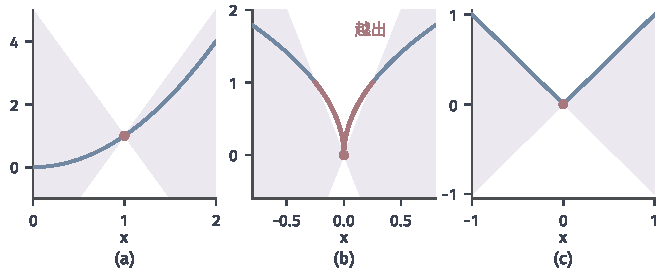
\includegraphics[width=112mm]{figures/06-differential-equations/01-ordinary-differential-equations/matplotlib/odeex-lipschitz-secants/figure.pdf}
  \caption{状态方向的Lipschitz条件。蓝线是函数图像，红点是基点，紫色区域是斜率$L$的双锥。(a)$x^2$在$[0,2]$上，基点$x=1$，$L=4$，图像在双锥内。(b)$2\sqrt{\lvert x\rvert}$，基点$x=0$，$L=4$，红色部分越出双锥；增大$L$只能缩小越出的范围，不能消除。(c)$\lvert x\rvert$，$L=1$，在基点不可微，图像仍在双锥内。}
  \label{fig:odeex-lipschitz-secants}
\end{BookInlineFigure}

图(a)的$x^2$在$[0,2]$上满足条件：
\[
 \lvert x^2-y^2\rvert=\lvert x+y\rvert\,\lvert x-y\rvert\leq4\lvert x-y\rvert.
\]
它在整条实轴上没有统一的$L$，这正是“局部”二字的用处。图(b)的$2\sqrt{\lvert x\rvert}$在原点不满足条件，这与多解的出现位置一致。图(c)说明Lipschitz条件比可微弱，折角并不妨碍它。

验证条件最常用的办法是求导。若$\partial_{\bm{x}}\bm{f}$存在且在$\bm{D}$上连续，在一个球形邻域内连接$\bm{x},\bm{y}$的线段上积分，得到
\[
 \bm{f}(t,\bm{x})-\bm{f}(t,\bm{y})
 =\int_0^1\partial_{\bm{x}}\bm{f}\bigl(t,\bm{y}+\theta(\bm{x}-\bm{y})\bigr)(\bm{x}-\bm{y})\,\mathrm{d}\theta.
\]
在紧邻域上取$L$为$\lVert\partial_{\bm{x}}\bm{f}\rVert_2$的最大值，就得到式~\eqref{eq:odeex-lipschitz}。

\paragraph{主要思想：积分方程是不动点问题}
积分方程~\eqref{eq:odeex-integral}把解刻画成一个自洽条件。给定一条曲线$\bm{u}$，沿它读出箭头，积分出一条新曲线，记为
\begin{equation}
 (\mathcal{T}\bm{u})(t)=\bm{x}_0+\int_{t_0}^{t}\bm{f}(s,\bm{u}(s))\,\mathrm{d}s.
 \label{eq:odeex-picard-map}
\end{equation}
解就是$\mathcal{T}$的不动点：把它代入，得到的还是它自己。把曲线看成无限维向量（每个时刻是一个坐标），$\mathcal{T}$是这个向量空间上的一个映射，初值问题就成了解方程$\bm{x}=\mathcal{T}\bm{x}$。

解这个方程最朴素的办法是反复代入。从常值曲线$\bm{x}^{(0)}(t)\equiv\bm{x}_0$出发，令
\begin{equation}
 \bm{x}^{(k+1)}=\mathcal{T}\bm{x}^{(k)},\quad k=0,1,\ldots,
 \label{eq:odeex-picard-iteration}
\end{equation}
这一列曲线称为\term{Picard迭代}（Picard iteration）。本节中上标$(k)$表示迭代次数，每个$\bm{x}^{(k)}$是一整条曲线。

\begin{example}[指数函数的Picard迭代]
\label{ex:odeex-picard-exp}
取$\dot x=x$，$x(0)=1$，此时$(\mathcal{T}u)(t)=1+\int_0^tu(s)\,\mathrm{d}s$。前几步分别是
\[
 x^{(0)}=1,\quad x^{(1)}=1+t,\quad x^{(2)}=1+t+\frac{t^2}{2}.
\]

设$x^{(k)}(t)=\sum_{j=0}^{k}t^j/j!$，代入式~\eqref{eq:odeex-picard-map}，逐项积分得到
\[
 x^{(k+1)}(t)=1+\sum_{j=0}^{k}\frac{t^{j+1}}{(j+1)!}=\sum_{j=0}^{k+1}\frac{t^j}{j!}.
\]
所以Picard迭代就是指数级数的部分和。在$[0,1]$上，余项满足
\[
 \lvert\mathrm{e}^t-x^{(k)}(t)\rvert\leq\frac{\mathrm{e}}{(k+1)!}.
\]
\end{example}

图~\ref{fig:odeex-picard-exp}显示，每迭代一次，曲线多贴合真解一段。对这个例子，迭代既不是在时间方向上推进，也不是逐点修正，而是每次把整条曲线替换一遍。

\begin{BookInlineFigure}
  \centering
  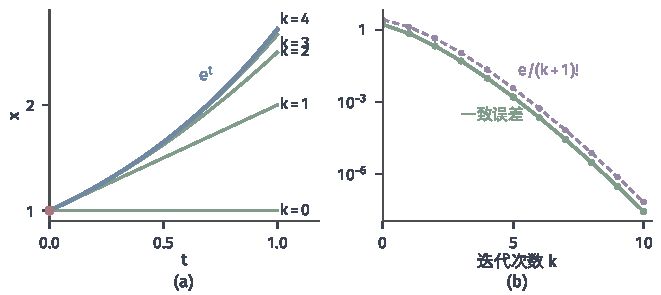
\includegraphics[width=112mm]{figures/06-differential-equations/01-ordinary-differential-equations/matplotlib/odeex-picard-exp/figure.pdf}
  \caption{$\dot x=x$，$x(0)=1$的Picard迭代。(a)绿线是$x^{(0)},\ldots,x^{(4)}$，蓝线是真解$\mathrm{e}^t$，红点是初值。(b)$[0,1]$上的一致误差（绿线）与上界$\mathrm{e}/(k+1)!$（紫色虚线），纵轴为对数坐标；衰减比任何几何级数都快。}
  \label{fig:odeex-picard-exp}
\end{BookInlineFigure}

\paragraph{为什么要缩短时间窗}
要保证迭代一般都收敛，自然想到压缩映射定理：完备度量空间上的压缩映射有唯一不动点，迭代从任何初值出发都收敛到它，可参考\BookChapterRef{chap:metric-space-maps}{卷四第3章“度量空间上的映射”}，那里也证明了区间上的连续函数在一致距离下完备。下面估计$\mathcal{T}$对曲线距离的作用。

设$\bm{u},\bm{v}$是两条曲线，$(s,\bm{u}(s))$和$(s,\bm{v}(s))$都在Lipschitz条件成立的盒子内。对$\lvert t-t_0\rvert\leq\delta$，由积分的范数不等式与式~\eqref{eq:odeex-lipschitz}，
\[
 \lVert(\mathcal{T}\bm{u})(t)-(\mathcal{T}\bm{v})(t)\rVert_2
 \leq\Bigl\lvert\int_{t_0}^{t}L\lVert\bm{u}(s)-\bm{v}(s)\rVert_2\,\mathrm{d}s\Bigr\rvert
 \leq L\delta\sup_{s}\lVert\bm{u}(s)-\bm{v}(s)\rVert_2.
\]

$\mathcal{T}$对距离的放大倍数至多是$L\delta$。积分把两条曲线的差沿时间累积，累积的时间越短，差就越小；$\delta$足够小时，这个映射就是压缩的。

图~\ref{fig:odeex-integral-smoothing}对$\dot x=x^2$，$x(0)=1$演示了这一点。两条任意选取的曲线在$[-1/8,1/8]$上一致距离约为$1.31$，经$\mathcal{T}$作用后，距离约为$0.125$，比值约$0.095$，小于这里的压缩常数$1/2$。

\begin{BookInlineFigure}
  \centering
  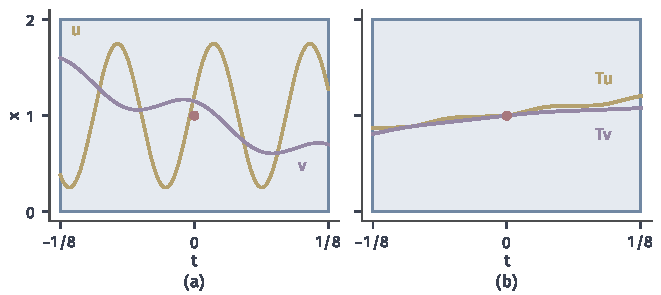
\includegraphics[width=112mm]{figures/06-differential-equations/01-ordinary-differential-equations/matplotlib/odeex-integral-smoothing/figure.pdf}
  \caption{积分映射缩小曲线距离。方程为$\dot x=x^2$，$x(0)=1$，浅蓝矩形是$\lvert t\rvert\leq1/8$、$\lvert x-1\rvert\leq1$的盒子。(a)盒内两条任取的曲线$u$（黄）和$v$（紫）。(b)它们的像$\mathcal{T}u$和$\mathcal{T}v$，都过红色初值点，振荡被积分抹平，一致距离由约$1.31$降为约$0.125$。}
  \label{fig:odeex-integral-smoothing}
\end{BookInlineFigure}

只缩短时间窗还不够，$\mathcal{T}$要把所选的曲线集合映回自身，否则迭代中途可能离开盒子，式~\eqref{eq:odeex-lipschitz}就不能再用。第~\ref{sec:odeex-local-existence}节的锥形估计恰好处理这件事。把这两个要求放在一起，就是\term{Picard--Lindelöf定理}（Picard--Lindelöf theorem）。

\begin{theorem}[Picard--Lindelöf定理]
\label{thm:odeex-picard-lindelof}
设$\bm{f}:\bm{D}\to\mathbb{R}^{n}$，$\bm{Q}=[t_0-a,t_0+a]\times\bm{B}_b\subseteq\bm{D}$，$\bm{f}$在$\bm{Q}$上连续，并存在$M,L>0$，使$\lVert\bm{f}\rVert_2\leq M$与式~\eqref{eq:odeex-lipschitz}在$\bm{Q}$上成立。令
\begin{equation}
 \delta=\min\Bigl\{a,\frac{b}{M},\frac{1}{2L}\Bigr\},\qquad I_\delta=[t_0-\delta,t_0+\delta].
 \label{eq:odeex-picard-window}
\end{equation}
则：
\begin{enumerate}
 \item 初值问题~\eqref{eq:odeex-ivp}在$I_\delta$上有经典解$\bm{x}$，其取值都在$\bm{B}_b$中；
 \item 若$I'\subseteq I_\delta$是含$t_0$的区间，$\bm{y}$是$I'$上的任一经典解，则$\bm{y}=\bm{x}$在$I'$上成立；
 \item Picard迭代~\eqref{eq:odeex-picard-iteration}在$I_\delta$上一致收敛到$\bm{x}$，且对$k\geq1$，
 \begin{equation}
 \lVert\bm{x}^{(k)}-\bm{x}\rVert_{\infty}\leq2^{1-k}\lVert\bm{x}^{(1)}-\bm{x}^{(0)}\rVert_{\infty},\qquad
 \lVert\bm{x}^{(k)}-\bm{x}\rVert_{\infty}\leq\lVert\bm{x}^{(k)}-\bm{x}^{(k-1)}\rVert_{\infty}.
 \label{eq:odeex-picard-error}
 \end{equation}
\end{enumerate}
\end{theorem}

\begin{proof}
\emph{选取空间。}记$\lVert\bm{y}\rVert_{\infty}$为$\lVert\bm{y}(t)\rVert_2$在$I_\delta$上的最大值，$C(I_\delta;\mathbb{R}^{n})$在这个范数下完备。令
\[
 \mathcal{X}=\bigl\{\bm{u}\in C(I_\delta;\mathbb{R}^{n}):\lVert\bm{u}(t)-\bm{x}_0\rVert_2\leq b,\ \forall t\in I_\delta\bigr\}.
\]
$\mathcal{X}$是闭集，一致收敛保持逐点的不等式，所以$\mathcal{X}$在一致距离下是完备度量空间；它含常值曲线$\bm{x}_0$，非空。

\emph{映回自身。}设$\bm{u}\in\mathcal{X}$。由$\delta\leq a$，点$(s,\bm{u}(s))$对$s\in I_\delta$都在$\bm{Q}$中，$s\mapsto\bm{f}(s,\bm{u}(s))$连续，积分有定义，$\mathcal{T}\bm{u}$连续。由$\delta\leq b/M$，
\[
 \lVert(\mathcal{T}\bm{u})(t)-\bm{x}_0\rVert_2
 \leq\Bigl\lvert\int_{t_0}^{t}\lVert\bm{f}(s,\bm{u}(s))\rVert_2\,\mathrm{d}s\Bigr\rvert
 \leq M\lvert t-t_0\rvert\leq b.
\]
所以$\mathcal{T}\bm{u}\in\mathcal{X}$。

\emph{压缩。}对$\bm{u},\bm{v}\in\mathcal{X}$，点$(s,\bm{u}(s)),(s,\bm{v}(s))$都在$\bm{Q}$中，前面的估计给出
\[
 \lVert\mathcal{T}\bm{u}-\mathcal{T}\bm{v}\rVert_{\infty}\leq L\delta\lVert\bm{u}-\bm{v}\rVert_{\infty}\leq\frac12\lVert\bm{u}-\bm{v}\rVert_{\infty}.
\]

\emph{不动点。}由压缩映射定理，$\mathcal{T}$在$\mathcal{X}$中有唯一不动点$\bm{x}$，Picard迭代从$\bm{x}^{(0)}\equiv\bm{x}_0\in\mathcal{X}$出发一致收敛到$\bm{x}$，其先验误差界和后验误差界取压缩常数$q=1/2$，就是式~\eqref{eq:odeex-picard-error}。不动点满足积分方程~\eqref{eq:odeex-integral}，因而是经典解。结论1和结论3得证。

\emph{任何解都留在盒内。}设$\bm{y}$是$I'$上的解。只看$t\geq t_0$的一侧，另一侧相同。令$t^\ast$为使$\bm{y}$在$[t_0,t]\cap I'$上取值于$\bm{B}_b$的$t$的上确界。在$[t_0,t^\ast)\cap I'$上点$(s,\bm{y}(s))$在$\bm{Q}$中，所以$\lVert\bm{y}(t)-\bm{x}_0\rVert_2\leq M(t-t_0)$在其上成立。

若$t^\ast$小于$I'$的右端点，则$t^\ast<t_0+\delta$，由连续性，
\[
 \lVert\bm{y}(t^\ast)-\bm{x}_0\rVert_2\leq M(t^\ast-t_0)<M\delta\leq b.
\]
这是严格不等式，$\bm{y}$在$t^\ast$之后一小段时间内还在球内，与上确界的定义矛盾。所以$\bm{y}$在$I'$上始终留在$\bm{B}_b$中。

\emph{唯一性。}两条解$\bm{x},\bm{y}$在$I'$上都留在盒内，都满足积分方程。记$e=\sup_{t\in I'}\lVert\bm{x}(t)-\bm{y}(t)\rVert_2$，它不超过$2b$，是有限数。相减并用式~\eqref{eq:odeex-lipschitz}，
\[
 \lVert\bm{x}(t)-\bm{y}(t)\rVert_2\leq L\delta\,e\leq\frac12e.
\]
对$t\in I'$取上确界，得$e\leq e/2$，即$e=0$，结论2得证。
\end{proof}

定理中各条件分工明确。$\bm{Q}\subseteq\bm{D}$让方程有定义；$\delta\leq b/M$让$\mathcal{T}$不把曲线带出盒子；$\delta\leq1/(2L)$让距离缩小；连续性让积分有定义，并使不动点是经典解。完备性保证迭代的柯西列有极限，这里用不到任何紧性。

\paragraph{计算过程}
Picard迭代的每一步都要计算一条曲线的积分，下面用$\dot x=x^2$，$x(0)=1$手算到第三轮，完整走一遍。取$a=1/2$，$b=1$，由图~\ref{fig:odeex-lipschitz-secants}(a)的计算，$M=4$，$L=4$，所以
\[
 \delta=\min\Bigl\{\frac12,\frac14,\frac18\Bigr\}=\frac18,\qquad q=L\delta=\frac12.
\]

\needspace{6\baselineskip}
\paragraph{变量}
\begin{itemize}
 \item $x^{(k)}$：第$k$轮的曲线，定义在$I_\delta=[-1/8,1/8]$上，例中都是多项式；
 \item $\Delta^{(k)}$：相邻两轮的一致距离$\lVert x^{(k)}-x^{(k-1)}\rVert_{\infty}$，用于后验误差界；
 \item $\varepsilon$：给定的误差容许值，例中取$2\times10^{-3}$。
\end{itemize}

\needspace{6\baselineskip}
\paragraph{初始化}
令$\bm{x}^{(0)}(t)\equiv\bm{x}_0$。例中$x^{(0)}=1$。

\needspace{6\baselineskip}
\paragraph{每轮更新}
对$k=0,1,\ldots$，依次执行：
\begin{enumerate}
 \item 由式~\eqref{eq:odeex-picard-iteration}，把$\bm{x}^{(k)}$代入右端并积分，得到$\bm{x}^{(k+1)}$。

 例中第一轮的被积函数是$1$，所以
 \[
 x^{(1)}(t)=1+t.
 \]
 第二轮对$(1+s)^2$积分，得到
 \[
 x^{(2)}(t)=1+t+t^2+\frac{t^3}{3}.
 \]
 第三轮对$(1+s+s^2+s^3/3)^2$积分，得到
 \[
 x^{(3)}(t)=1+t+t^2+t^3+\frac23t^4+\frac13t^5+\frac19t^6+\frac{1}{63}t^7.
 \]
 \item 计算$\Delta^{(k+1)}$。例中相邻两轮的差都在$t=1/8$处取到最大模，于是
 \[
 \Delta^{(1)}=\frac18,\quad \Delta^{(2)}\approx1.63\times10^{-2},\quad \Delta^{(3)}\approx1.48\times10^{-3}.
 \]
 \item 若后验误差界$q\Delta^{(k+1)}/(1-q)$不超过$\varepsilon$，就停止，否则继续。由式~\eqref{eq:odeex-picard-error}，$q=1/2$时这个界就是$\Delta^{(k+1)}$。

 例中$\Delta^{(2)}>\varepsilon$，第二轮后继续；$\Delta^{(3)}\leq\varepsilon$，第三轮后停止。
\end{enumerate}

最终得到$x^{(3)}$，它在$[-1/8,1/8]$上与真解的误差被保证不超过$1.48\times10^{-3}$。实际误差约为$1.06\times10^{-4}$，比界小一个数量级。

图~\ref{fig:odeex-picard-square}(a)显示迭代在时间窗内很快贴合真解，窗外贴合得较慢，越靠近真解的奇点$t=1$差得越远。图(b)比较实际误差和先验界$2^{1-k}\cdot1/8$，先验界用的是全局的$q=1/2$，实际误差衰减得快得多。

\begin{BookInlineFigure}
  \centering
  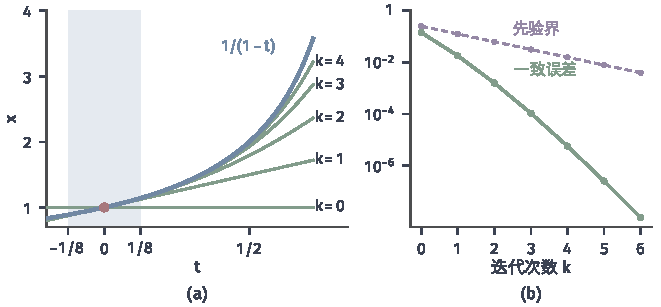
\includegraphics[width=112mm]{figures/06-differential-equations/01-ordinary-differential-equations/matplotlib/odeex-picard-square/figure.pdf}
  \caption{$\dot x=x^2$，$x(0)=1$的Picard迭代。(a)绿线是$x^{(0)},\ldots,x^{(4)}$，蓝线是真解，浅蓝带是时间窗$[-1/8,1/8]$。(b)时间窗上的一致误差（绿线）与先验界$2^{1-k}\cdot\tfrac18$（紫色虚线），纵轴为对数坐标。}
  \label{fig:odeex-picard-square}
\end{BookInlineFigure}

\paragraph{时间窗不必缩到$1/(2L)$}
定理中的$1/(2L)$是为了让$\mathcal{T}$在一步之内就成为压缩映射。例~\ref{ex:odeex-picard-exp}在$[0,1]$上有$L\delta=1$，不是压缩，迭代却收敛得比几何级数还快。原因是误差要累积多次才会放大，而累积的时间区域越来越窄。

设$\delta'=\min\{a,b/M\}$，定义域换成$I_{\delta'}$。前面“映回自身”的论证只用了$\delta'\leq a$与$\delta'\leq b/M$，所以$\mathcal{T}$仍把相应的$\mathcal{X}$映回自身，迭代都有定义。下面对$k\geq0$归纳证明，对$t\in I_{\delta'}$，
\begin{equation}
 \lVert\bm{x}^{(k+1)}(t)-\bm{x}^{(k)}(t)\rVert_2\leq\frac{ML^{k}\lvert t-t_0\rvert^{k+1}}{(k+1)!}.
 \label{eq:odeex-picard-factorial}
\end{equation}

$k=0$时，左端是$\bm{f}(s,\bm{x}_0)$积分的范数，被积函数的范数不超过$M$，所以不超过$M\lvert t-t_0\rvert$。设$k-1$时成立，对$t\geq t_0$，由式~\eqref{eq:odeex-lipschitz}，
\[
 \lVert\bm{x}^{(k+1)}(t)-\bm{x}^{(k)}(t)\rVert_2
 \leq L\int_{t_0}^{t}\frac{ML^{k-1}(s-t_0)^{k}}{k!}\,\mathrm{d}s
 =\frac{ML^{k}(t-t_0)^{k+1}}{(k+1)!}.
\]
$t<t_0$的情形相同。

式~\eqref{eq:odeex-picard-factorial}的右端对$k$求和收敛，和不超过$M(\mathrm{e}^{L\delta'}-1)/L$，所以$\bm{x}^{(k)}$一致收敛，其极限是$\mathcal{T}$的不动点。两个不动点的差用同样的归纳，得到对任意$k$，
\[
 \lVert\bm{u}(t)-\bm{v}(t)\rVert_2\leq2b\,\frac{(L\lvert t-t_0\rvert)^{k}}{k!},
\]
令$k\to\infty$，差为零。任何解都留在盒内的论证也只用到$\delta'\leq b/M$。因此解在整个$I_{\delta'}$上存在且唯一，时间窗的长度由$a$和$b/M$决定，不受$L$限制；$L$只影响收敛的快慢。

\paragraph{Lipschitz条件只是充分条件}
定理给出的是唯一性的充分条件，并不必要。考虑方向相反的方程
\[
 \dot x=-2\operatorname{sgn}(x)\sqrt{\lvert x\rvert}.
\]
它在原点同样不满足Lipschitz条件。但右端关于$x$单调不增，两条解$u,v$之差满足
\[
 \frac{\mathrm{d}}{\mathrm{d}t}(u-v)^2=2(u-v)\bigl(f(u)-f(v)\bigr)\leq0.
\]
所以差只会减小，初值相同的两条解在$t$增大的方向上不会分开，向前唯一。

图~\ref{fig:odeex-one-sided-merge}显示了这个方程的解：从$x_0$出发的解是$\operatorname{sgn}(x_0)(\sqrt{\lvert x_0\rvert}-t)^2$，在$t=\sqrt{\lvert x_0\rvert}$到达零线后停在那里，不同的解在有限时间内合并。把时间倒过来，方程变成式~\eqref{eq:odeex-sqrt}的奇函数版本，从零线出发可以有多条解，所以向后不唯一。这里的唯一性来自单调性，与Lipschitz条件无关。

\begin{BookInlineFigure}
  \centering
  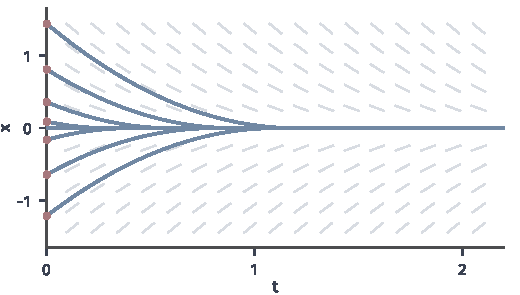
\includegraphics[width=88mm]{figures/06-differential-equations/01-ordinary-differential-equations/matplotlib/odeex-one-sided-merge/figure.pdf}
  \caption{$\dot x=-2\operatorname{sgn}(x)\sqrt{\lvert x\rvert}$的解。短线是方向场，红点是不同的初值，蓝线是相应的解，在有限时间内汇入零线。向前的解由初值确定，向后从零线出发则有多个可能。}
  \label{fig:odeex-one-sided-merge}
\end{BookInlineFigure}

\paragraph{Lipschitz常数要对时间局部一致}
定义~\ref{def:odeex-local-lipschitz}要求$L$在邻域内对时间一致。如果每个时刻各有一个常数，但常数随时间无界，唯一性也会失败。令$\operatorname{clip}(x;0,t^2)$表示把$x$截断到$[0,t^2]$，定义
\begin{equation}
 f(t,x)=\begin{cases}\dfrac{2}{t}\operatorname{clip}(x;0,t^2),&t>0,\\0,&t\leq0.\end{cases}
 \label{eq:odeex-clip}
\end{equation}

由$0\leq\operatorname{clip}\leq t^2$，有$\lvert f(t,x)\rvert\leq2t$，所以$f$在$t=0$处连续，从而在$\mathbb{R}^{2}$上连续。固定$t>0$，$f$关于$x$是Lipschitz的，常数为$2/t$；固定$t\leq0$，$f$恒为零。每个时刻单独看都满足条件，但常数$2/t$在$t\to0$时无界。

对每个$c\in[0,1]$，曲线$x=ct^2$满足$0\leq x\leq t^2$，右端等于$2ct$，恰是它的导数。所以从$x(0)=0$出发有无穷多条解，如图~\ref{fig:odeex-time-lipschitz}所示。两条解的差以$2/t$的相对速率增长，这个速率在$t=0$附近的积分发散，足以从零差产生非零差。

\begin{BookInlineFigure}
  \centering
  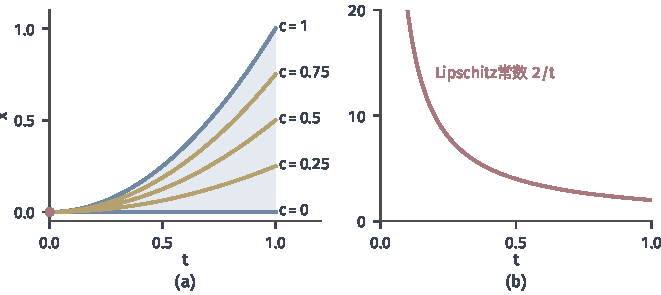
\includegraphics[width=112mm]{figures/06-differential-equations/01-ordinary-differential-equations/matplotlib/odeex-time-lipschitz/figure.pdf}
  \caption{Lipschitz常数对时间不一致导致多解。(a)方程~\eqref{eq:odeex-clip}的解$x=ct^2$，浅蓝区域$0\leq x\leq t^2$内，$c$取$0,0.25,0.5,0.75,1$，都从红点出发。(b)固定时刻的Lipschitz常数$2/t$，在$t\to0$时无界。}
  \label{fig:odeex-time-lipschitz}
\end{BookInlineFigure}

\paragraph{紧性与完备性}
Peano和Picard两条路线用的工具不同，结论的强弱也不同，表~\ref{tab:odeex-peano-picard}把它们放在一起。

\begin{BookInlineTable}
  \centering
  \caption{两条存在性路线的对比}
  \label{tab:odeex-peano-picard}
  \begin{tabular}{lll}
    \toprule
     & Peano路线 & Picard路线 \\
    \midrule
    右端条件 & 连续 & 连续，状态方向Lipschitz \\
    逼近对象 & Euler折线 & Picard迭代 \\
    收敛来源 & 紧性，只有子列 & 完备性，整列收敛 \\
    结论 & 至少一个解 & 恰有一个解，有误差界 \\
    无限维空间 & 可能无解 & 证明不变，结论成立 \\
    \bottomrule
  \end{tabular}
\end{BookInlineTable}

最后一行值得注意。Picard路线只用到空间的完备性和范数不等式，状态空间换成任何完备的赋范空间，证明的步骤不变，只需假设盒子上$\bm{f}$有界且满足Lipschitz条件。第~\ref{sec:odeex-local-existence}节$c_0$上的反例恰好不满足Lipschitz条件。
